\documentclass[journal]{IEEEtran}
% IEEE Robotics and Automation Letters (RA-L) format.
\IEEEoverridecommandlockouts
\usepackage{cite}


%%%% Customized packages
\usepackage[table]{xcolor}
\usepackage{amssymb}
\usepackage{amsmath}
\usepackage{bm}
\usepackage{rotating}
% \usepackage{geometry} % removed: IEEEtran manages page geometry for RA-L
\usepackage[position=bottom]{subfig}
% \usepackage{subcaption}	
% \usepackage{subfigure}
% \usepackage{natbib}
\usepackage{tabularx,booktabs,caption,ragged2e}
\usepackage{graphics, wrapfig}

\DeclareMathOperator{\E}{\mathbb{E}}
\DeclareMathOperator{\R}{\mathbb{R}}
\usepackage{graphicx}

\newcommand{\magpie}{\raisebox{-0.2em}{
\includegraphics[height=1.2em]{magpie.pdf}}}

% hyperref must be loaded last
\usepackage{url}
\usepackage[hidelinks]{hyperref}

\title{\magpie MAGPIE: Multi-Primitive Bimanual Garment Folding from Crumpled States with Pixel-based Flow Matching Policies}


% The \applicant macro works with any number of applicants. There are two
% commands used to separate the names and addresses of multiple
% applicants: \And and \AND.
%
% Using \And between applicants leaves it to LaTeX to determine where to
% break the lines. Using \AND forces a line break at that point. So,
% if LaTeX puts 3 of 4 applicants names on the first line, and the last
% on the second line, try using \AND instead of \And before the third
% applicant name.

% NOTE: applicants will be visible only in the camera-ready and preprint versions (i.e., when using the option 'final' or 'preprint'). 
% 	For the initial submission the applicants will be anonymized.

\author{Halid Abdulrahim Kadi$^{1,2}$, Houdeyfa Ajrou$^{3}$, Lucy Walsh$^{1}$, Ivan Kapelyukh$^{4}$,
        Kasim Terzi{\'c}$^{5}$, and John Oyekan$^{1,2}$% <-this % stops a space
\thanks{Manuscript received: \today. This work was supported by the
Engineering and Physical Sciences Research Council, United Kingdom, under
the grant ``A digital COgnitive architecture to achieve Rapid Task
programming and flEXibility in manufacturing robots through human
demonstrations'' (DIGI-CORTEX, EP/W014688/2).}%
\thanks{$^{1}$Department of Computer Science, University of York, United Kingdom.}%
\thanks{$^{2}$Department of Computer Science, Loughborough University, United
Kingdom; Halid Abdulrahim Kadi and John Oyekan were with the University of
York while part of this work was conducted. (e-mail:
\texttt{halidkadi.robot@gmail.com}).}%
\thanks{$^{3}$Department of Computer Science, University of Sheffield, United Kingdom.}%
\thanks{$^{4}$Department of Computing, Imperial College London, United Kingdom.}%
\thanks{$^{5}$School of Computer Science, University of St Andrews, United Kingdom.}%
\thanks{Digital Object Identifier (DOI): see top of this page.}}


\begin{document}

\markboth{IEEE Robotics and Automation Letters. Preprint Version.}%
{Kadi \MakeLowercase{\textit{et al.}}: MAGPIE: Multi-Primitive Bimanual Garment Folding from Crumpled States}

\maketitle
%===============================================================================
%===============================================================================
\begin{abstract}

Garment manipulation remains one of the most challenging tasks in robotic control due to the large degrees of freedom, severe self-occlusions, and complex underactuated dynamics of cloth objects. Recent data-driven approaches fragment the manipulation pipeline into multi-primitive setups, typically employing Reinforcement Learning (RL) for flattening and Imitation Learning (IL) or heuristics for folding. However, folding garments from arbitrary crumpled configurations within a unified end-to-end learning-based method has remained elusive. We present MAGPIE, a unified, bimanual, multi-primitive method that uses a flow matching policy for primitive parameter inference. We also propose central-alignment tasks, where MAGPIE aligns a crumpled garment towards an arbitrary flattened target position within the workspace; this is especially essential for downstream ironing tasks. Our simulation and real-world experiments demonstrate that MAGPIE achieves state-of-the-art flattening and folding success rates directly from crumpled states across diverse garments.
\end{abstract}

\begin{IEEEkeywords}
Deformable object manipulation, dual-arm manipulation, imitation learning, flow matching, garment folding.
\end{IEEEkeywords}

\IEEEpeerreviewmaketitle

\section{Introduction}

Robotic manipulation of cloth-like deformable objects presents a significant technical challenge with profound societal and economic implications \cite{kadi2023data}. Automating cloth handling is essential for high-volume garment manufacturing \cite{nayak2018introduction}, and assistive care for elderly and mobility-impaired populations \cite{ohneberg2023assistive}. Despite this broad demand, reliable robotic cloth handling remains exceptionally difficult; garments confound traditional control through a high-dimensional state space, severe self-occlusions, and highly underactuated physical dynamics \cite{xue2023unifolding}.

Consequently, the garment manipulation literature has historically divided the control pipeline into isolated subtasks: flattening and downstream folding. A pervasive methodological split has emerged to address these distinct phases in the multi-primitive control setup. For flattening, Deep Reinforcement Learning (DRL) is heavily favoured \cite{canberk2022cloth, avigal2022speedfolding, ha2022flingbot}; this is because formulating a geometric coverage reward is relatively straightforward, whereas collecting comprehensive human demonstrations across near-infinite crumpled states for Imitation Learning (IL) is intractable. Conversely, for the folding phase, the paradigm flips---formulating a dense RL reward for heavily self-occluded, folded geometries is notoriously difficult \cite{kadi2025lagarnet}, prompting researchers to rely on IL or heuristic template/keypoint-based approaches \cite{barbany2025bifold}. While stitching together these separate policies can yield functional systems \cite{avigal2022speedfolding, canberk2022cloth, xue2023unifolding}, they rely on disjointed classifiers and complex heuristic switching. Consequently, they are inherently brittle---if a garment deforms or a fold fails mid-execution, the agent typically cannot recover or switch back to a flattening primitive without resetting the entire pipeline.


In this paper, we resolve the above challenges through unifying the two processes with a multi-primitive imitation learning framework that can be learned in a strict end-to-end manner. Our method, MAGPIE (\textbf{M}ulti-primitive \textbf{A}pproach for \textbf{G}arment manipulation with \textbf{P}ixel-based \textbf{I}mitation l\textbf{E}arning), bypasses intractable RL exploration by directly cloning human expert strategies. It resolves IL's compounding error by learning both \textit{which} behavioural primitive to execute and \textit{how} to continuously parameterise it directly from visual observations. To achieve efficient, stable learning, we ground our policy in Conditioned Optimal Transport Flow Matching (COT-FM) \cite{lipman2022flow, black2024pi0}, mitigating the slow and highly curved inference trajectories of standard diffusion models \cite{chi2025diffusion}. In general, our main contributions are as follows:
\begin{enumerate}
    \item We propose MAGPIE, a unified, end-to-end, hierarchical data-driven method that bridges flattening and folding under a single multi-primitive Imitation Learning framework.

    \item We synthesise the dual-arm garment manipulation literature with the Parameterised Action Markov Decision Process (PA-MDP) control literature, adapting COT-FM to coordinate discrete primitive selection and continuous parameter generation while mitigating mode collapse.

    \item We propose central-alignment tasks, where the policy flattens and aligns the garment towards a target position around the intersection between dual arms, in contrast to conventional canonicalisation-alignment tasks \cite{avigal2022speedfolding, xue2023unifolding, canberk2022cloth}.

    \item We evaluate our system in both simulation and reality, demonstrating that MAGPIE folds a wide variety of previously unseen garment categories and transfers to real-world setups in a zero-shot manner.
\end{enumerate}


\section{Related Work}

We define garment shaping as a long-horizon, hierarchical process comprising flattening and downstream folding, where flattening includes the conventional canonicalisation-alignment tasks \cite{canberk2022cloth} and our proposed central-alignment task.

\subsection{Data-driven Methods in Dual-Arm Garment Manipulation}
\label{sec:dual_arm_shaping}

Data-driven garment manipulation generally falls into two paradigms: learning continuous, low-level end-effector control \cite{black2024pi0, chi2025diffusion}, or inferring parameters for predefined behavioural primitives \cite{ha2022flingbot, avigal2022speedfolding}. We align with the latter, employing primitives like dual-arm pick-and-fling and pick-and-place to handle the complex dynamics of cloth. Crucially, the choice of state representation significantly impacts policy robustness. While physics-based meshes or dense point clouds are popular \cite{wu2024unigarmentmanip}, they are computationally complex to estimate under severe occlusion and often introduce a massive simulation-to-reality gap; semantic keypoints provide succinct topological structures \cite{deng2025clasp}, yet often require domain-specific foundation models or structural priors. MAGPIE bypasses these complexities by utilising pure top-down RGB images, inferring semantic structures directly without heavy point-cloud processing or explicit skeleton matching.

\paragraph{Reinforcement Learning for Flattening} Deep Reinforcement Learning (DRL) dominates the initial flattening phase. Methods like FlingBot \cite{ha2022flingbot}, SpeedFolding \cite{avigal2022speedfolding}, ClothFunnels \cite{canberk2022cloth}, and ClothMate \cite{luo2025clothmate} predominantly employ Spatial Action Value Maps (SAVMs) \cite{lee2021learning} to discretise the action space. To respect strict kinematic reachability limits, they mask the action heatmap or drag the garment into the operable workspace \cite{xue2023unifolding}. However, extending SAVM-based DRL to the downstream folding phase is notoriously intractable; the severe self-occlusions inherent to folded geometries fundamentally confound dense reward formulation.

\paragraph{Imitation Learning for Folding} The literature instead pivots to Imitation Learning (IL) \cite{kadi2025draper} or heuristic methods \cite{canberk2022cloth} for the folding phase. Systems such as BiFold \cite{barbany2025bifold} generate spatial folding parameters from step-wise linguistic prompts or predefined keypoint templates. While these methods can execute complex folds from perfectly flattened initialisations, they struggle to recover autonomously if the garment deforms, snags, or shifts mid-execution, requiring a complete manual reset of the pipeline.

\paragraph{Unified Flattening and Folding Systems} Attempts to unify these disparate processes have yielded functional but highly engineered systems. UniFolding \cite{xue2023unifolding} uses dedicated, hard-coded network classifiers to trigger transitions between flattening primitives (trained via RL) and folding primitives (trained via IL); this rigid phase switching prevents seamlessly mixing primitives if a mistake needs correcting mid-fold. Alternatively, UniGarmentManip \cite{wu2024unigarmentmanip} learns cross-deformation structural correspondences on point clouds to replay human demonstrations across garments, yet demands substantial engineering overhead for skeleton extraction and pre-processing. In contrast, MAGPIE eliminates hard-coded phase classifiers and complex geometric pre-processing, unifying primitive selection and parameterisation in a cohesive, end-to-end visual framework.

\subsection{Data-Driven Multi-Primitive Methods for Manipulation}
\label{sec:multi_primitive_control}

In robotic control, complex, long-horizon tasks are typically decomposed into elemental control modules, or action primitives, coordinated either via the Options framework over Semi-Markov Decision Processes (SMDPs) \cite{sutton1999between} or via Parameterised Action Markov Decision Processes (PA-MDPs) \cite{masson2016reinforcement} (Section \ref{sec:PA-MDP}). SMDP-based methods learn the low-level intra-option motor control concurrently, which introduces immense sample complexity for highly deformable objects. By associating predefined, discrete behavioural primitives (e.g., \textit{fling}, \textit{place}) with continuous spatial parameters, PA-MDPs abstract away low-level motor control. This makes the framework exceptionally well-suited for dual-arm garment manipulation, where the primary challenge is spatial reasoning rather than trajectory generation.

Within PA-MDPs, DRL algorithms like MAPLE \cite{nasiriany2022augmenting} and HACMan++ \cite{jiang2024hacman++} optimise the joint discrete-continuous action space. However, when the discrete choice of primitives is multiplied by the high-dimensional parameters required for dual-arm coordination across near-infinite crumpled garment states, online RL struggles significantly with sample inefficiency, local optima, and an intractable exploration burden. Consequently, we adopt Imitation Learning (IL) to solve the PA-MDP formulation, leveraging human demonstrations to directly supervise both the discrete selection and the continuous parameterisation. Multi-primitive IL approaches, such as HDR-IL \cite{xie2020deep} and PRIME \cite{gao2024prime}, extract complex sequences directly from expert trajectories; however, they rely heavily on historical state-action relationships or millions of transitions to train an Inverse Dynamics Model (IDM). In contrast, MAGPIE posits that for highly deformable objects, historical context is less informative than a precise topological estimation of the immediate visual state, inferring the optimal primitive directly from the current visual observation embedding.

\subsection{Generative Imitation Learning for Manipulation}
\label{sec:diffusion_policies}

Recent advancements in Behavioural Cloning (BC) integrate generative modelling to resolve the multimodal action distribution issues that previously limited direct Multi-Layer Perceptron (MLP) methods. While diffusion-like policies \cite{chi2025diffusion} and Action Chunking with Transformers (ACT) \cite{zhao2023learning} excel at continuous end-effector control, their iterative denoising processes form highly curved probability trajectories. This translates to slow convergence, high inference latency, and a marked sensitivity to execution noise \cite{black2024pi0}, which compound across primitive transitions in multi-step garment shaping.

Flow Matching \cite{lipman2022flow} addresses these exact bottlenecks; grounded in optimal transport theory, flow models directly regress the vector field of a probability path via Ordinary Differential Equations (ODEs). This defines straight-line optimal transport flows, substantially reducing the number of required inference steps while offering superior stability and generalisation \cite{zhang2025flowpolicy}. Frameworks such as Flow Policy \cite{zhang2025flowpolicy} and state-of-the-art VLA models like $\pi_0$ \cite{black2024pi0} leverage these efficiencies for highly reactive, robust low-level manipulation. However, the application of flow matching within explicit multi-primitive architectures remains largely unexplored. MAGPIE bridges this gap by adapting Conditioned Optimal Transport Flow Matching (COT-FM) to a multi-primitive framework, constraining the flow generation to continuous spatial parameters of predefined primitives. This establishes a highly efficient, unified generative policy capable of flattening and folding diverse garments directly from fully crumpled states.


\section{Preliminaries} \label{sec:preliminaries}

We adopt the partially observable Markov decision process (POMDP) \cite{kaelbling1998planning} augmented with action parameterisation \cite{masson2016reinforcement}, collectively referred to as the Parameterised Action POMDP (PA-POMDP), as our mathematical formulation.

\subsection{Parameterised Action Partially Observable Markov Decision Process (PA-POMDP)} \label{sec:PA-MDP}

A Markov Decision Process (MDP) models a stochastic decision system as a five-tuple $(\mathcal{S}, \mathcal{A}, \mathcal{P}, \mathcal{R}, \rho_0)$, comprising the state space, action space, transition probability $\mathcal{P}(s' \mid s, a)$, reward function, and initial state distribution. A POMDP extends this to a seven-tuple $(\mathcal{S}, \mathcal{A}, \mathcal{P}, \mathcal{R}, \rho_0, \mathcal{X}, \mathcal{O})$, where the true state $s \in \mathcal{S}$ is not directly observable; instead, the agent receives an observation $x \in \mathcal{X}$ with probability $\mathcal{O}(x \mid s)$.

In robotics, policies are often developed over a discrete set of action primitives $\Omega$ that enable the robot to perform semantically meaningful behaviours in the environment. Formally, each primitive $\omega \in \Omega$ is represented by a control module $\mathcal{C}_\omega(a^{\omega})$, where $a^{\omega} \in \mathbb{R}^{d_{\omega}}$ signifies the continuous input parameters defined within the parameter dimension $d_{\omega}$. The Parameterised Action MDP (PA-MDP) \cite{masson2016reinforcement} incorporates such action primitives, where the agent selects a parameterised action $a \equiv (\omega, a^{\omega}) \in \mathcal{A}$, comprising the primitive type and its corresponding continuous parameters.

\subsection{Action Primitives} \label{sec:action_primitives}

MAGPIE adopts four types of primitives essential for effective and robust performance. Each primitive is parameterised by a set of normalised 2-D pixel coordinates in $[-1, 1]$ (a total of $4$, $8$, $4$, and $0$ parameters, respectively), which are de-normalised and projected onto the table plane before execution.

\paragraph{Pick-and-Fling:} Primarily utilised for highly crumpled states or garment reorientation, the action flips the garment's orientation, reveals hidden key-points, and helps untangle the cloth; it is parameterised by one 2-D grasp point per arm ($4$ values).

\paragraph{Dual-arm pick-and-place:} Essential for precise folding and for adjusting the garment after initial flattening; intersecting arm trajectories are executed sequentially to prevent self-collisions. It is parameterised by a 2-D pick and a 2-D place point per arm ($8$ values).

\paragraph{Single-arm pick-and-place:} Also known as the \textit{drag} primitive, it brings the garment toward the intersection of the dual-arm workspace and performs fine-grained adjustments, such as aligning trouser legs that fall outside the shared reachable area ($4$ values).

\paragraph{No Operation:} The robot arms remain stationary, allowing the system to stabilise upon successfully completing the task ($0$-dimensional).

\subsection{Optimal Transport Conditional Flow Matching for Policy Learning} \label{sec:ot_cfm}

Flow matching provides a robust generative framework by constructing continuous-time normalising flows via vector field regression \cite{lipman2022flow}. In the context of robotic policy learning, the objective is to model a conditional action distribution $p_1(a \mid x)$ given an environment observation $x$. To achieve this, Lipman et al. \cite{lipman2022flow} formulate an Ordinary Differential Equation (ODE) that smoothly transports samples from a tractable prior Gaussian noise distribution $p_0$ into the complex, observation-conditioned target data distribution $p_1(\cdot \mid x)$:
\begin{equation}
    \frac{da_k}{dk} = v_\theta(a_k, k \mid x)
\end{equation}
where $v_\theta$ is the learned vector field parameterised by $\theta$ and conditioned on the current observation $x$, and $a_k$ represents the action state at time $k$ \cite{lipman2022flow}. 

Conditional Optimal Transport Flow Matching (COT-FM) simplifies this objective by sampling the intermediate action $a_k$ from the deterministic linear interpolant $a_k = k a_1 + (1 - k) a_0$ for $k \in [0, 1]$, which minimises the transport cost between the noise and target distributions. Because this path is a straight line, the ground-truth velocity is simply the constant vector $v_{\text{gt}}(a_k, k) = \frac{da_k}{dk} = a_1 - a_0$, requiring no computationally expensive ODE simulation during training. By sampling observation-action pairs $(x, a_1)$ from the expert demonstration dataset $\mathcal{D}$, the network minimises the expected mean squared error between its predicted, observation-conditioned vector field and this ground-truth velocity:
\begin{equation}
    \mathcal{L}_{\text{FM}} = \mathbb{E}_{\substack{k \sim \mathcal{U}[0,1], \\ a_0 \sim p_0, a_1 \sim \mathcal{D}\\ a_k \sim p(a_k \mid a_1, k)}} \left\| v_\theta(a_k, k \mid x) - (a_1 - a_0) \right\|^2
\end{equation}

\begin{figure*}[t]
\centering
\subfloat[Network architecture.]{%
    
\includegraphics[width=0.82\linewidth]{plots/Magpie-architecture.jpg}%
    \label{fig:architecture}}\\[4pt]
\subfloat[Data sampling and augmentation.]{%
    \raisebox{\dimexpr-\height}{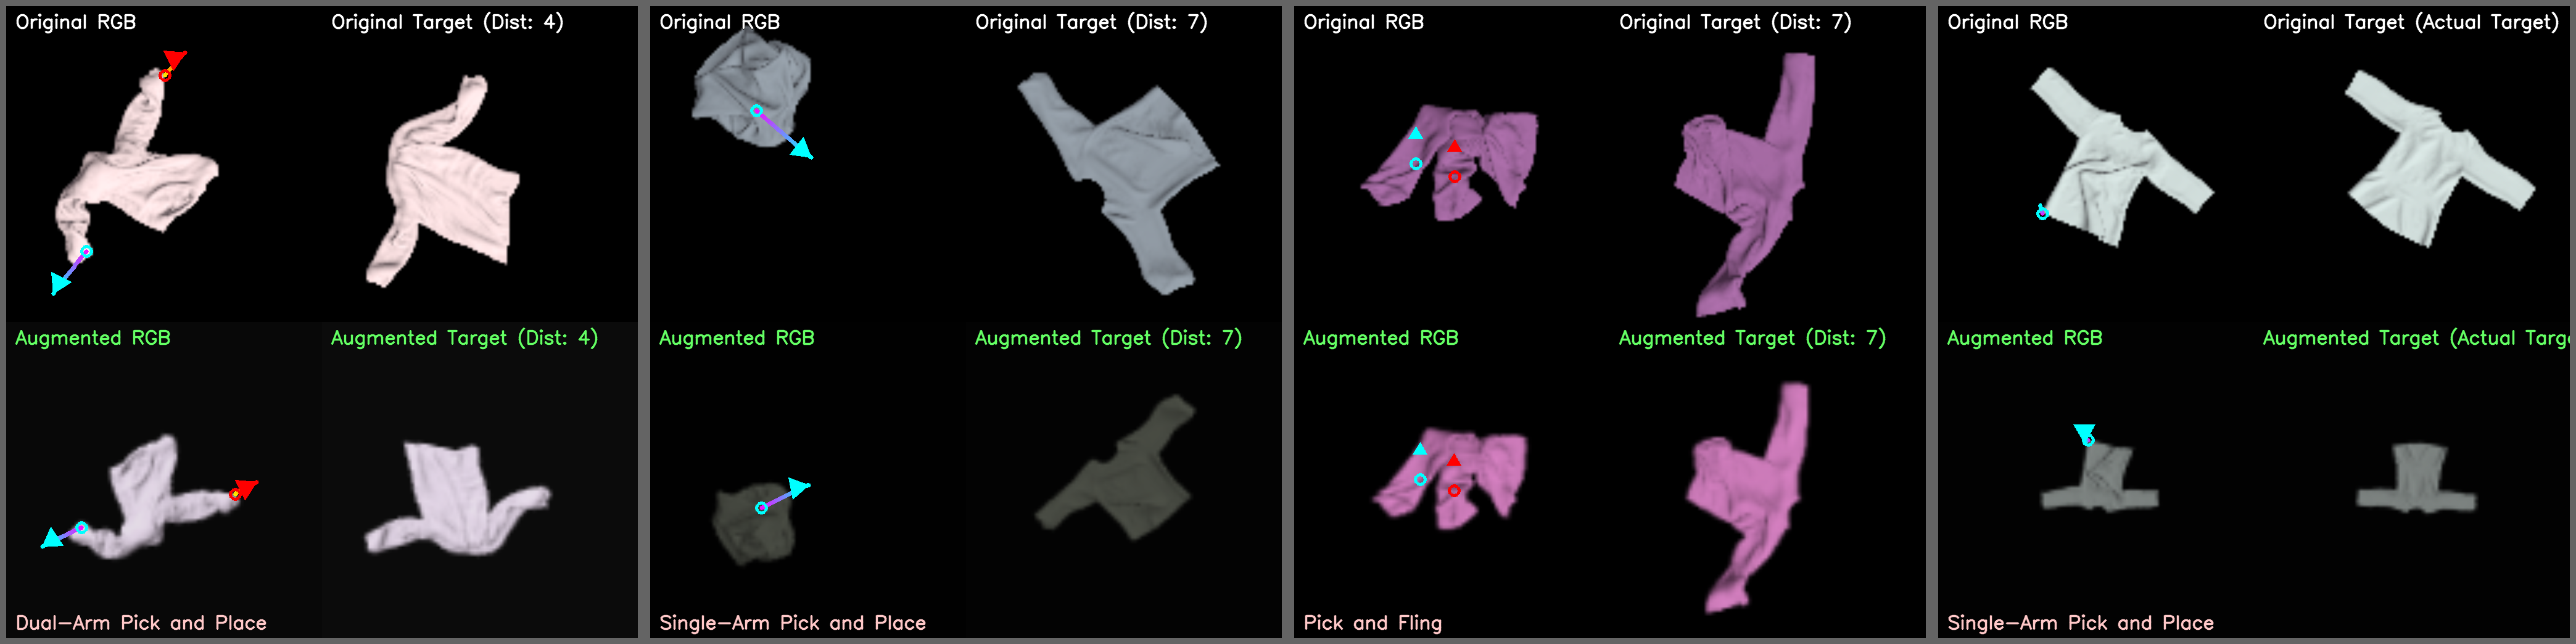
\includegraphics[width=0.61\linewidth, trim=0 0 2088bp 0, clip]{plots/dataloader_augment_master_multi_batch.png}}%
    \label{fig:data_augmentation}}\hfill
\subfloat[Human demonstration interface.]{%
    \raisebox{\dimexpr-\height}{\begin{minipage}[b]{0.38\linewidth}
    \centering
    
\includegraphics[width=\linewidth]{plots/human-interface-initial.png}\\[2pt]
    
\includegraphics[width=\linewidth]{plots/human-interface-success.png}%
    \end{minipage}}%
    \label{fig:human_interface}}
\caption{Overview of MAGPIE. (a) The multi-primitive network architecture; the resulting action is snapped to the corresponding workspace, and the pick action onto the cloth mask, before environment execution. (b) The data sampling and augmentation pipeline; augmentation includes rotation, flipping, scaling, colour jittering, RGB channel permutation and gripper-swapping, whilst hindsight sampling randomly selects future target states as well as the actual target of the trajectory. (c) The interface used to collect human demonstrations and to run the human baseline (initial state, top; a successful fold, bottom).}
\label{fig:overview}
\end{figure*}

\section{Method} \label{sec:method}

We build MAGPIE upon the PA-POMDP framework (Section \ref{sec:PA-MDP}), utilising top-down RGB current and goal images as observations alongside multiple action primitives. An MLP-based classification network predicts the appropriate primitive for the current state (Section \ref{sec:classification}), whilst a suite of primitive-specific COT-FM policies infers the corresponding continuous action parameters (Section \ref{sec:cot_fm_learning}); see Figure \ref{fig:architecture}. To improve learning efficiency, we train MAGPIE with future-state goal sampling inspired by Hindsight Experience Replay (HER) \cite{andrychowicz2017hindsight} (Section \ref{sec:data_aug}). Finally, we sequence the flattening and folding behaviours using a vision-based heuristic relying on normalised coverage and alignment Intersection over Union (IoU). The method is developed in simulation and successfully transferred to the real world in a zero-shot manner.

\subsection{Multi-Primitive Learning as Classification}
\label{sec:classification}

Our method, MAGPIE, decouples the high-level primitive selection from the low-level action parameter generation. We employ an MLP-based classification network $f_\theta$ that maps the latent state $z$ to a predicted primitive $\omega = \arg\max_k f_{\theta}(z)_k$. To address the severe imbalance between demonstrated primitives in our dataset, we optimise the network using a weighted cross-entropy loss:
$$\mathcal{L}_{cls}(\theta) = - \sum_{\omega \in \Omega} \lambda_\omega y_\omega \log(\hat{y}_\omega)$$
where $y_\omega \in \{0, 1\}$ is the ground-truth binary indicator for primitive $\omega$, $\hat{y}_\omega$ is the predicted probability from the network, and $\lambda_\omega$ denotes the empirical class weight used to penalise majority classes. 

Once the optimal primitive $\omega^*$ is identified, the latent visual embedding $z$ is routed exclusively to the designated generative network corresponding to $\omega^*$. Detailed architectural specifications for this classification network are provided in Appendix \ref{app:architecture}.

\subsection{Primitive Parameter Learning via COT-FM Policy}
\label{sec:cot_fm_learning}

We utilise COT-FM \cite{black2024pi0, lipman2022flow} (detailed in Section \ref{sec:ot_cfm}) to model the generative mapping from an initial noise distribution to the target action parameter distribution. Rather than employing a single one-size-fits-all network conditioned on a one-hot encoding, we instantiate independent vector field networks $v_{\phi}^{\omega}(a_k^\omega, k \mid z)$ for each primitive type $\omega \in \Omega$. Each is trained with the flow matching objective of Section \ref{sec:ot_cfm}---denoted $\mathcal{L}_{para}^{\omega}(\phi)$---conditioned on the latent embedding $z$ and sampling $a_1$ from the demonstration subset $\mathcal{D}^\omega$ where primitive $\omega$ was executed. This architectural split effectively prevents mode collapse and parameter interference across distinctly different robotic behaviours; we demonstrate its empirical superiority via ablation studies. The exact implementation details of these policy networks are given in Appendix \ref{app:architecture}.

\subsection{Data Augmentation and Future-State Goal Sampling}
\label{sec:data_aug}
To improve data efficiency and provide a dense, reachable learning signal, we actively sample future states for goal conditioning during training. Rather than conditioning the policy strictly on the terminal goal state of an episode, we dynamically sample a future observation $x_{goal}$ from a randomly selected future time step $t + \Delta t$ within the same trajectory sequence. This acts as a proximal sub-goal, effectively bridging the severe visual distribution shift between highly crumpled initial states and perfectly folded final states. By anchoring the generative policy to near-term geometric changes, the network learns local spatial transformations much faster. This future-state relabelling is directly inspired by Hindsight Experience Replay (HER)~\cite{andrychowicz2017hindsight}, which similarly converts partial rollouts into successful goal-reaching demonstrations.

Furthermore, to ensure robustness to visual perturbations and bridge the simulation-to-reality gap, we apply an aggressive suite of spatial and visual data augmentations to the RGB observations prior to latent encoding (Figure~\ref{fig:data_augmentation}). These include color jittering (modifying brightness, contrast, saturation, and hue), random channel permutation, random vertical flipping (with corresponding inversions of spatial action coordinates), random scaling within a $[0.7, 1.0]$ range, and random rotations in $1^\circ$ increments. To handle the symmetrical nature of dual-arm manipulation, we also employ an action-swapping augmentation with a $50\%$ probability, which geometrically mirrors the observation and remaps the corresponding left/right arm action parameters.

\subsection{Training Details}
All network components—including the shared visual encoder, the primitive classification network, and the suite of flow-matching action generative models—are optimised jointly in an end-to-end manner via the weighted objective $\mathcal{L}_{total} = \beta_{prim} \mathcal{L}_{prim} + \beta_{para} \sum_{\omega \in \Omega} \mathcal{L}_{para}^{\omega}$, with the coefficients empirically set to $\beta_{prim} = 0.01$ and $\beta_{para} = 1.0$. We employ the AdamW optimiser and apply weighted cross-entropy to handle the highly imbalanced distribution of primitives within the demonstration dataset. Our dataset comprises 200 simulation episodes for each garment category, and 40 real-world episodes for each physical garment instance; each episode is rolled out to a maximum of 20 steps. A complete breakdown of all hyperparameters, network architectures, and environment configurations can be found in Appendix \ref{app:architecture}.



\section{Experiments}
\label{sec:experiments}

We evaluate MAGPIE in both simulation and the real world to answer three core research questions. \textbf{RQ1} (Section \ref{sec:exp_sota}): how does MAGPIE compare to state-of-the-art (SoTA) domain-specific flattening and folding baselines? \textbf{RQ2} (Section \ref{sec:exp_abl}): what do MAGPIE's architectural components and training-data composition individually contribute? \textbf{RQ3} (Section \ref{sec:exp_real_world}): how effectively does the simulation-trained policy transfer to the real world?

\subsection{Comparison Against SoTA Garment Manipulation Systems}
\label{sec:exp_sota}

We benchmark MAGPIE in simulation against the non-unified baselines ClothFunnels \cite{canberk2022cloth} and ClothMate \cite{luo2025clothmate}, and the unified baseline UniFolding \cite{xue2023unifolding}; we exclude methods that rely on step-wise language instructions to ensure a fair comparison.

\paragraph{Simulation Experimental Setup}
We build our simulation environment upon the ClothFunnels variant of the SoftGym benchmark \cite{lin2020softgym}, powered by the PyFlex physics engine \cite{li2018learning}, sourcing realistic garment meshes (long-sleeve T-shirts, trousers, skirts, and dresses) from the Cloth3D dataset \cite{bertiche2020cloth3d}. For each category, our dataset comprises 200 training episodes mixing ``hard'' (highly crumpled) and ``easy'' (semi-flattened) initial states, plus 30 validation and 30 evaluation episodes that strictly use ``hard'' initialisations, following the ClothFunnels methodology. For our novel central-alignment and folding tasks, we explicitly align workspace radii, dual-arm base placements, camera configurations, fabric stiffness, and cloth particle radii with our real-world setup; a side-by-side parameter comparison (Table \ref{tab:sim-real-params}) and detailed simulation mechanics are deferred to Appendices \ref{sec:real-world-setup} and \ref{app:architecture}.

\paragraph{Task Setups} We evaluate three simulated tasks. For each episode the target geometry is produced once by rolling out a scripted keypoint demonstrator and cached, so every method is scored against identical goals. In \emph{Canonicalisation-Alignment}, a crumpled garment must be flattened into a fixed canonical pose; \emph{Central-Alignment} shares this objective with a workspace-centred target pose and is evaluated across all garment categories. \emph{Goal-Directed Folding} requires a two-step fold executed \emph{through} the canonicalisation-alignment state, i.e. an ordered set of $K=3$ subgoals: the flattened/canonical state $S_0$, fold-1 $S_1$, and fold-2 $S_2$. The alignment tasks use a $20$-step horizon and folding a $25$-step horizon, both without early stopping; full metric definitions and success criteria are provided in Appendix~\ref{app:eval_protocol}.



\paragraph{Metrics} For the alignment tasks, we report Normalised Coverage (NC), Normalised Improvement (NI), Alignment IoU (A-IoU, direct mask overlap with no re-alignment), and the Success Rate (SR) of reaching $\text{NC}>80\%$ and $\text{A-IoU}>70\%$, cross-trajectory (C-SR) and at the last step (LS-SR). For folding, we report Mean Particle Distance (MPD) \cite{canberk2022cloth}, A-IoU, Max IoU (overlap maximised over a rigid 2D transform), and the Sequential IoU-Based Success Rate (Sq-IoU-SR) of reproducing the ordered fold subgoals $S_0,\dots,S_{K-1}$. All metrics are taken at the final trajectory step; full definitions are given in Appendix~\ref{app:eval_protocol}.



\begin{figure*}[!t]
    \centering
    \subfloat[Qualitative comparison of MAGPIE against SoTA bimanual flattening methods on the Canonicalisation-Alignment Task, starting from a highly crumpled out-of-distribution initial state and terminating at the target aligned state.]{%
        
\includegraphics[width=0.75\linewidth]{plots/traj_canon_alignment.png}%
        \label{fig:qualitative_sota_canon}}\\[4pt]
    \subfloat[Qualitative performance of MAGPIE on the Central-Alignment Task across different garment categories.]{%
        
\includegraphics[width=0.75\linewidth]{plots/traj_central_alignment.png}%
        \label{fig:qualitative_central_garment}}
    \caption{Qualitative execution sequences on (a) the Canonicalisation-Alignment and (b) the Central-Alignment tasks.}
    \label{fig:qualitative_traj}
\end{figure*}

\begin{figure*}[!t]
    \centering
    \subfloat[Canonicalisation-Alignment Task across various methods]{%
        
\includegraphics[width=0.63\linewidth]{plots/metrics_2x2_heatmap.png}%
        \label{fig:canon_heatmap}}
    \subfloat[Central-Alignment Task across garment categories.]{%
        
\includegraphics[width=0.35\linewidth]{plots/magpie_garment_radar_plot.png}%
        \label{fig:central_radar}}
    \caption{Quantitative results: (a) canonicalisation-alignment comparison against SoTA methods and the human baseline (full numerical results in Table \ref{tab:longsleeve-flattening}, Appendix \ref{app:eval_protocol}); (b) MAGPIE's central-alignment generalisation across garment categories.}
    \label{fig:quant_alignment}
\end{figure*}

% --- EXPERIMENT ANALYSIS PLACEHOLDER ---
\paragraph{Experiment Design} We first analyse comparative performance on canonicalisation-alignment (Figures \ref{fig:qualitative_sota_canon} and \ref{fig:canon_heatmap}; full numbers in Table \ref{tab:longsleeve-flattening}, Appendix \ref{app:eval_protocol}), then MAGPIE's alignment generalisation across garment categories (Figures \ref{fig:qualitative_central_garment} and \ref{fig:central_radar}), and finally its downstream folding proficiency on long-sleeve garments.


\subsection{Goal-Directed Folding in Simulation}
\label{sec:exp_folding}

We now evaluate MAGPIE's core competency: producing neat, structured folds directly from crumpled states. In \textit{goal-directed folding}, a long-sleeve garment must be manipulated from a highly crumpled configuration, through the canonicalisation-alignment state, into a demonstrated two-step fold; success requires reproducing the ordered sequence of folded geometries, making the task substantially more sensitive to compounding errors and self-occlusion. We evaluate every method over 30 held-out ``hard'' initialisations and report the folding metrics defined above.

We compare: \textbf{MAGPIE (All-Garment)}, our full unified policy; \textbf{MAGPIE (Long-sleeve, Folding-only)}, trained exclusively on long-sleeve folding demonstrations \emph{without} goal conditioning or hindsight sampling; \textbf{MAGPIE + Heuristic Folding}, in which the All-Garment policy flattens the garment before a deterministic keypoint-based heuristic folder \cite{canberk2022cloth, xue2023unifolding} executes the folds; and \textbf{Human}, an operator using the demonstration interface (Figure~\ref{fig:human_interface}) as an upper-bound reference.

\begin{table}[!t]
\caption{Goal-directed folding in simulation on long-sleeve garments (30 hard crumpled initialisations, two-step fold through canonicalisation-alignment). Distances are reported in normalised units; higher is better for A-IoU, Max IoU, and Sq-IoU-SR, lower is better for MPD. \textbf{TODO: populate with final numbers.}}
\label{tab:sim-folding}
\centering
\small
\begin{tabular}{l|ccc||c}
\toprule
 & \multicolumn{3}{c||}{\textbf{MAGPIE}} & \\
\cmidrule(lr){2-4}
\textbf{Metric} & \textbf{All-Garment} & \textbf{LS-only} & \textbf{+\,Heuristic} & \textbf{Human} \\
\midrule
MPD $\downarrow$        & -- & -- & -- & -- \\
A-IoU $\uparrow$        & -- & -- & -- & -- \\
Max IoU $\uparrow$      & -- & -- & -- & -- \\
Sq-IoU-SR $\uparrow$    & -- & -- & -- & -- \\
\bottomrule
\end{tabular}
\end{table}

\begin{figure}[!t]
    \centering
    % 
\includegraphics[width=1.0\linewidth]{plots/traj_folding_cmp.png}
    \caption{Qualitative comparison of goal-directed folding in simulation. Each row tracks the execution sequence from a crumpled long-sleeve initial state, through the canonicalisation-alignment sub-goal, to the final two-step fold, for the All-Garment MAGPIE policy, the long-sleeve folding-only variant, the MAGPIE~+~heuristic hand-off, and the human operator. \textbf{TODO: add rendered trajectory grid.}}
    \label{fig:qualitative_folding}
\end{figure}

Table~\ref{tab:sim-folding} and Figure~\ref{fig:qualitative_folding} report the comparison. We expect the All-Garment policy to benefit from goal conditioning and hindsight sampling, and to match or exceed the heuristic hand-off by seamlessly interleaving flattening and folding primitives.
% --- FOLDING RESULTS ANALYSIS PLACEHOLDER ---
[Placeholder: Detailed quantitative analysis of the goal-directed folding results, including per-metric comparison, failure modes of the heuristic hand-off, and the gap to human performance.]


\subsection{Ablation Studies}
\label{sec:exp_abl}

We systematically ablate MAGPIE's core components in simulation on the long-sleeve central-alignment task, employing the setup and metrics of Section \ref{sec:exp_sota}.

We rigorously isolate the performance contributions of MAGPIE's design choices. \textbf{Primitive Routing}: we compare our decoupled networks against a \textbf{Flat Policy} (predicting continuous primitive bins $[-1, 1]$ alongside its parameters), a \textbf{OneHot Policy} (a single master parameter network conditioned on one-hot primitive encodings), and an \textbf{Ordinal Policy} (conditioned via scaled ordinal encodings); these baselines adopt a one-size-fits-all parameter formulation and mask non-effective entries as zeros. \textbf{Policy Architecture Backbone}: we replace the COT-FM backend with a standard \textbf{Diffusion Policy} (100 denoising steps) and a deterministic \textbf{Direct Action Policy} with MSE loss utilising a similar architectural footprint. \textbf{Data Composition}: we compare our full multi-garment dataset against single-category training sets, as well as ablating the hindsight sampling and data augmentations.

\begin{figure}[!h]
    \centering
    % \includegraphics[width=1.0\linewidth]{plots/ablation_results.png}
    \caption{Ablation study results isolating the impact of flow-matching routing, semantic representation learning, alternative generative backbones, and data distribution across 50 evaluation seeds. (Plots detail metric comparisons for Routing, Backbone, and Data Composition).}
    \label{fig:ablations}
\end{figure}

% --- ABLATION RESULTS PLACEHOLDER ---
[Placeholder: Detailed quantitative analysis of ablation results.]


\subsection{Real-World Deployment}
\label{sec:exp_real_world}

We deploy MAGPIE on a physical bimanual robotic system to evaluate its sim-to-real transfer. As long-sleeve T-shirts are structurally the most complex category to manipulate, we restrict our physical folding evaluations to this garment type.

\begin{figure}[!h]
    \centering
    % \includegraphics[width=1.0\linewidth]{plots/real_world_setup.png}
    \caption{Physical workspace configuration. The dual-arm cell utilises a UR5e and UR16e equipped with OnRobot RG2 grippers. A static, centrally-mounted RealSense D435i camera provides RGB observations for policy inference.}
    \label{fig:real_world_setup}
\end{figure}

\paragraph{Real World Setup} 
As visualised in Figure \ref{fig:real_world_setup}, we employ a UR5e and a UR16e robot with OnRobot RG2 grippers, observed by a static RealSense D435i camera mounted centrally at approximately 1.65~m in an eye-to-hand configuration. The policy relies solely on RGB frames; the control pipeline utilises the UR-RTDE package \cite{urrtde2025} for Cartesian trajectory execution. Calibrated transforms and workspace parameters are given in Appendix \ref{sec:real-world-setup}.

\paragraph{Evaluation Metrics}
We use the same vision-based metrics as in simulation, reporting only A-IoU and Sq-IoU-SR for folding, as particle-level tracking is unavailable. We test end-to-end folding of our T-shirt-specialised policy on 5 physical T-shirts of varying colour, scale, and shape, with 10 consecutive trials each from fully crumpled states (50 executions). For goal-conditioned canonical alignment, we assess the general policy across 5 garment categories, each from 8 initial orientations with 5 trials per orientation (200 trials).

\begin{figure}[!h]
    \centering
    % \includegraphics[width=1.0\linewidth]{plots/real_world_deployment.png}
    \caption{Real-world execution of MAGPIE. The sequence illustrates the transition from a highly crumpled T-shirt to a canonical alignment, followed by a subsequent 2-step fold.}
    \label{fig:real_world}
\end{figure}

% --- REAL WORLD RESULTS PLACEHOLDER ---
[Placeholder: Comprehensive analysis of physical deployment results. Discussion on the sim-to-real transfer efficiency, observed failure modes during physical execution (e.g., gripper slip, fabric friction), and the overall success rates for both canonical alignment (across all garments) and end-to-end folding (long-sleeve garments).]

\section{Discussion}
\label{sec:discussion}

The primary advantage of MAGPIE lies in its ability to split high-level structural categorisation from low-level geometric parameter generation. By elevating the generative policy to operate over structured primitive action parameters rather than unconstrained, step-by-step end-effector positions, we drastically reduce exploration complexity and mitigate the compounding errors that plague pure pixel-to-action networks.

While continuous pixel-to-action diffusion policies \cite{chi2025diffusion} show promise in short-horizon, single-arm behaviours, applying standard generative architectures to multi-primitive, multi-arm configurations introduces severe training instabilities. The discrete classification of high-level primitives typically converges orders of magnitude faster than the continuous spatial distribution generation; this mismatch triggers mode collapse, where the agent repeatedly outputs safe, majority-class primitives while ignoring necessary high-momentum actions like flinging. MAGPIE's decoupled routing structure natively isolates these vector fields, keeping the flow-matching gradients independent and preventing behaviour interference. Furthermore, its local, fully open architecture naturally integrates workspace-specific dual-arm kinematic boundaries without the brittle prompting techniques typical of closed, API-bound commercial Vision-Language-Action frameworks.

\paragraph{Limitations}
Despite achieving high alignment scores, a core limitation of our framework is its reliance on 2D visual metrics like Normalised Coverage (NC) and Intersection-over-Union (IoU) to judge geometric correctness. For instance, garments with wide geometric profiles (e.g., flared skirts or loose dresses) can assume highly warped or sub-optimally folded interior states while still completely filling out the bounding area of the target mask. In these edge cases, high NC and IoU metrics decouple from actual visual neatness, exposing the limitations of purely mask-based objective functions.

\paragraph{Future Work}
Future directions will focus on broadening the validation envelope to encompass out-of-distribution, complex multi-layered garments and unseen fabric blends. We intend to integrate real-time tactile and force-torque feedback into the COT-FM integration steps, allowing the policy to dynamically sense fabric tension and friction during high-speed flinging, further reducing the sim-to-real gap. As MAGPIE relies on specific goal images to drive the policy, adding language-to-goal generation would enable more general types of folding and flattening. Finally, since this work employs traditional MLP and CNN structures, we will investigate transformer-based backbones.

\section{Conclusion}
\label{sec:conclusion}

In this paper, we introduced MAGPIE, a unified multi-primitive framework for long-horizon dual-arm garment manipulation. By formalising the cloth alignment and folding sequence as a PA-POMDP and decoupling discrete primitive routing from continuous spatial parameter generation using independent COT-FM networks, our approach successfully avoids policy mode collapse and behavioural interference. Enhanced by dynamic future-state goal sampling inspired by Hindsight Experience Replay, MAGPIE demonstrates superior sample efficiency and robustness over state-of-the-art deformable baselines. Finally, physical hardware deployments confirm that MAGPIE successfully bridges the simulation-to-reality gap, providing a scalable path forward for autonomous, multi-arm fabric manipulation.

\section*{Acknowledgment}
We would like to thank the Institute of Safe Autonomy at the University of York for hosting the experimental evaluations, where \textbf{Dr James Hilder} and \textbf{Dr Rob Woolley} assisted us in setting up the robot platform. We also acknowledge the use of the Viking cluster at York. This work was supported by the Engineering and Physical Sciences Research Council, United Kingdom, under the grant DIGI-CORTEX (EP/W014688/2).

\bibliographystyle{IEEEtran}
\bibliography{example}

\newpage

\appendices

\section{Network Architecture and Implementation Details}
\label{app:architecture}

This appendix details the exact network architecture and training configuration of MAGPIE; we refer the reader to Section~\ref{sec:method} for the conceptual overview. Our implementation relies on a highly decoupled architecture to manage the multi-primitive nature of garment shaping: a shared vision encoder feeds an MLP primitive classifier and a suite of primitive-specific MLP-based flow-matching networks.

\subsection{Shared Vision Encoder}
To process visual inputs, we utilise a ResNet-18 backbone~\cite{he2016deep}. Because standard Batch Normalisation performs poorly with the small batch sizes typical of continuous robotic control algorithms, we replace all 2D Batch Normalisation layers with Group Normalisation (\texttt{num\_groups}=16). The final fully connected layer is removed, and an Adaptive Average Pooling layer compresses the spatial features into a 512-dimensional vector.

To refine these features for downstream tasks, this vector is subsequently passed through an MLP projector consisting of two hidden layers with dimensions $[512, 512]$ and GELU activations, outputting a final 512-dimensional visual embedding. During training, a feature noise factor of $0.05$ is applied to the observation features to improve robustness. For state-inclusive experiments, physical vector states are concatenated with this projected visual embedding.

\subsection{Primitive Classification Head}
The high-level primitive selection is handled by an MLP classifier. The network takes the 512-dimensional projected visual embedding and passes it through two hidden layers with dimensions $[256, 128]$. We apply a ReLU activation function, followed by Layer Normalisation and a Dropout layer with a probability of $p = 0.5$. The final output maps to the $K=4$ available action primitives. To ensure balanced decision-making during training, the classes are equally weighted ($\lambda_\omega = 1.0$ for all classes).


\begin{table}[!t]
\centering
\caption{Hyperparameters for MAGPIE Training}
\label{tab:hyperparameters}
\begin{tabular}{lc}
\toprule
\textbf{Hyperparameter} & \textbf{Value} \\
\midrule
\multicolumn{2}{c}{\textit{Optimisation}} \\
\midrule
Optimiser & AdamW \\
Learning Rate & $3 \times 10^{-4}$ \\
Weight Decay & $1 \times 10^{-2}$ \\
Batch Size & 1024 \\
Total Update Steps & 120,000 \\
Trial Validation Interval & 5,000 \\
EMA Decay Rate & 0.9999 \\
Warmup Steps & 3,000 \\
\midrule
\multicolumn{2}{c}{\textit{Flow Matching \& Architecture}} \\
\midrule
Inference Iterations & 4 \\
Flow-Matching Backbone & MLP (\texttt{ConditionalMLP1D}) \\
Backbone Hidden Dims & $[1024, 1024, 1024, 512]$ \\
Backbone Activation & GELU \\
Vision Encoder & ResNet-18 (\texttt{original}) \\
Observation Embedding Dim & 512 (Projected) \\
Input Modalities & \texttt{rgb} + \texttt{goal\_rgb} \\
Input Image Resolution & $128 \times 128$ \\
Observation Horizon & 1 \\
Prediction / Action Horizon & 1 \\
Action Dimension & 4, 8, 4, 0 \\
\midrule
\multicolumn{2}{c}{\textit{Primitive Classification Network}} \\
\midrule
Primitive Integration & Separate Networks \\
Hidden Dimensions & $[256, 128]$ \\
Activation & ReLU \\
Dropout & 0.5 \\
Normalisation & LayerNorm \\
Class Weights & $[1.0, 1.0, 1.0, 1.0]$ \\
Primitive Loss Weight ($\beta_{prim}$) & 0.01 \\
\bottomrule
\end{tabular}
\end{table}



\subsection{Conditioned Flow-Matching Networks (COT-FM)}
For each of the $K$ primitives, we instantiate an independent MLP backbone (\texttt{ConditionalMLP1D}) to regress the optimal transport vector field. This separate-network integration ensures that distinct robotic behaviours do not suffer from parameter interference. The no-operation primitive carries no continuous parameters (dimension $0$) and therefore has no associated network.
\begin{itemize}
    \item \textbf{Architecture Backbone:} Each network flattens the (single-step) action into a vector and passes it through a stack of dense layers with hidden dimensions $[1024, 1024, 1024, 512]$, GELU activations, and dropout $0.1$, regressing the vector field over the primitive's continuous action dimension ($4$, $8$, or $4$). Unlike a temporal U-Net, this backbone contains no convolutions or spatial down-/up-sampling.
    \item \textbf{Timestep Embedding:} The continuous flow timestep $k$ is encoded using Sinusoidal Positional Embeddings (dimension $256$), which are then passed through a two-layer MLP sequence (Linear $\rightarrow$ Mish $\rightarrow$ Linear) to generate the temporal feature.
    \item \textbf{Conditioning:} Conditioning is applied by concatenation: the global visual context $z$ and the timestep feature are concatenated with the flattened noisy action and fed jointly to the dense network, which directly regresses the velocity field.
    \item \textbf{Integration:} During training, the flow matches the constant velocity field $a_1 - a_0$. During inference, we integrate the learned field with a $4$-step Euler ODE solver to transport the initial Gaussian noise into the predicted spatial parameters.
\end{itemize}

\subsection{Optimization Hyperparameters}
We optimise all networks end-to-end using the AdamW optimiser with a base learning rate of $3 \times 10^{-4}$ and a weight decay of $1 \times 10^{-2}$. We employ a cosine annealing learning rate scheduler with a warmup period of 3,000 steps. To stabilise training, we apply gradient clipping and maintain an Exponential Moving Average (EMA) of the model weights with a high decay rate of 0.9999.


\section{Integration of Other Methods}
We do not re-implement the baselines. Instead, we take each author's released code and adapt it to our framework. This keeps the comparison focused on the manipulation policy rather than the surrounding system. Every baseline reads the same top-down observation. Every baseline emits actions in our normalised pixel primitive space (\texttt{pick-and-fling}, single/dual \texttt{pick-and-place}, and \texttt{no-op}), with coordinates in $[-1,1]$. We grant each baseline the same environment-provided per-arm reachability masks. We also evaluate each one on the same tasks, initial states, and cached goals. For every baseline we first summarise the original method, then describe how we adapt its code.

\subsection{ClothFunnels: Method, Architecture, Training and Inference}
Cloth Funnels~\cite{canberk2022cloth} learns a \emph{canonicalised-alignment} objective. The objective funnels crumpled configurations into a narrow set of structured, fully-visible canonical poses, such as a T-shape for shirts, at a fixed 2D position and orientation. Simple heuristics can then fold the garment. The method parameterises manipulation as spatial action maps. It augments the $128{\times}128$ top-down RGB observation with a two-channel scale-invariant positional encoding. It then transforms this input across $16$ rotations and $6$ scales ($\{0.75,1.0,1.5,2.0,2.5,3.0\}$), giving $96$ inputs. A fully-convolutional value network predicts a dense per-pixel value map for every transform and each of two primitives: a dynamic dual-arm \texttt{pick-and-fling} and a quasi-static \texttt{pick-and-place}. The method factorises the reward as $R_{CA}=(1-\alpha)R_{C}+\alpha R_{A}$ ($\alpha=0.6$). The canonicalisation term $R_{C}$ measures per-vertex distance to the best-aligned goal, and the alignment term $R_{A}$ measures the residual rigid-transform error. The network uses one encoder per reward term, each with a decoder head per primitive. It trains self-supervised in simulation over roughly $12.5$k episodes, regressing each action's delta-reward $\Delta R_{CA}$ with an MSE loss under $\epsilon$-greedy exploration. At inference it scores every (rotation, scale, pixel) triple, masks out infeasible actions, and executes the arg-max. It recovers the pick and place pixels by inverting the chosen rotation-and-scale transform. A separate convolutional keypoint detector then supplies the landmarks for the final heuristic fold.

\subsection{ClothFunnels: Integration into Our Framework}
We move the action discretisation out of the environment and into the policy. The released code then outputs continuous coordinates in our normalised pixel space. This maps its dynamic unfolding and static placement onto our continuous bimanual and single-arm manoeuvres. The original code folds with a 3D inverse-kinematic heuristic. We replace this heuristic with a purely planar 2D formulation. We split the original unified fold into a fixed sequence: two single-arm placements, then one simultaneous dual-arm manipulation. We also feed the environment's exact per-arm reachability masks into the policy, which replaces its own coarse approximations.

The policy runs on a $480 \times 480$ observation from a downward-facing camera at two metres. We downsample and crop this observation to $128 \times 128$ for the network. The code keeps three coordinate frames to handle this crop and the rotational augmentations: a tightly cropped transformed space, a rotated pre-transformed space, and the absolute original space. We use the absolute original space to reorient the dynamic actions. This makes the fling drive the fabric upward in the frame rather than sideways as in the original setup. The policy selects its unfolding actions from the peaks of the spatial action-value maps. After $10$ flattening steps, a convolutional keypoint detector locates six semantic landmarks (the shoulders, sleeves, and hem) and computes the final fold.

The detector isolates six landmarks: the left and right shoulders, the top-left and top-right collar vertices, and the bottom-left and bottom-right hem vertices. The pipeline uses these landmarks only in the terminal phase. Once unfolding and flattening finish, the six keypoints anchor a deterministic fold. The shoulders and top corners set the inward sleeve fold, and the bottom hem keypoints set the final upward fold towards the collar. The six keypoints therefore act as absolute waypoints for the terminal fold.

\subsection{ClothMate: Method, Architecture, Training and Inference}
ClothMate~\cite{luo2025clothmate} flattens garments from arbitrary configurations in a generalisable, data-efficient way. Its key insight is grasp--fling consistency: grasping the same point pair produces a consistent fling response regardless of the current crumpled state. It exploits this insight with a two-stage design. First it learns point-wise fling responses under a canonicalised, aligned configuration. Then it generalises to arbitrary states through a point-to-point projection. This design decouples state estimation from action prediction. The decoupling tames the infinite-DOF dynamics and self-occlusion of garments and improves data efficiency across categories. A spatial-action-map value network, as in Cloth Funnels, scores dynamic \texttt{fling} and \texttt{place} candidates over $16$ rotations at $128{\times}128$ resolution. It blends rigid and deformable value predictions, and we set the deformable weight to $0.4$. A U-Net predicts four garment-corner keypoints through a heatmap head and a garment-state score through a classification head. A low relative-coverage-area (RCA) reading switches the policy from flinging to a keypoint-driven bimanual \texttt{pick-and-stretch} that tensions the most contracted edge. It trains the value network self-supervised and supervises the U-Net on annotated corners and states. At inference it flings until the garment is spread, then parameterises an open-loop stretch from the four corners.

\subsection{ClothMate: Integration into Our Framework}
Our ClothMate adaptation reuses the masking and coordinate handling of our Cloth Funnels adaptation. To refine the terminal flattening, it swaps the two single-arm placements for one bimanual stretch; this \texttt{pick-and-stretch} resembles our dual-arm pick-and-place primitive (Section \ref{sec:action_primitives}), as does the \texttt{fold} primitive of UniFolding \cite{xue2023unifolding}. The spatial policy network then handles only the high-velocity dynamic unfolding.

A binary state classifier governs the switch from flinging to stretching. It reads the fabric's spatial arrangement and triggers the stretch only when the relative coverage area (RCA) score drops below $0.15$, which marks a sufficiently spread garment. A second check guards against bad grasps. The U-Net classifier branch must also report a confidence above $0.45$ before the stretch runs.

The four U-Net corners drive validation and parameterisation during flattening, not a terminal fold. When the classifier flags a spread garment, the code measures the horizontal distances between the keypoint pairs. This measurement serves two purposes. It first classifies the garment's gross morphology, separating trousers from upper-body garments so the stretch avoids over-tensioning constrained parts like waistbands. It then finds the most contracted, wrinkled edge. Finally, the four corners set the anchor constraints and directions for a safe, open-loop bimanual stretch.

\subsection{UniFolding: Method, Architecture, Training and Inference}
UniFolding~\cite{xue2023unifolding} unifies unfolding and folding in one policy, UFONet, that acts directly on a partial garment point cloud masked from RGB-D. The point-cloud input improves generalisation and reduces sensitivity to texture and shape. A sparse-convolution ResUNet3D encoder produces a $128$-d global feature and per-point $128$-d features, and a self-attention module refines them. Three heads consume these features. An action-classification head decides the unfolding-to-folding transition from the global feature. A fling head regresses $K$ grasp-keypoint candidates by attention-based offset voting in the canonical NOCS frame, which exploits garment bilateral symmetry, and a pairwise MLP then ranks the keypoint pairs. A pick-and-place head predicts the dual-arm pick and place points for fold-1 and fold-2, and a drag primitive covers unreachable grasps. Training is sample-efficient and human-centric. It uses offline Virtual-Reality demonstrations ($\sim$16\,h across long- and short-sleeve shirts), a self-supervised simulation stage that trains the pairwise scoring head, and an online real-world human-in-the-loop stage with pairwise-preference annotations. The losses combine a variety (minimum-over-$N$) loss and a smooth-$L_1$ loss for the keypoints and pick/place, plus a cross-entropy loss on the preferences. At inference it classifies the stage, scores fling keypoint pairs for unfolding or pick/place points for folding, and runs them as dual-arm $\mathrm{SE}(3)$ actions.

\subsection{UniFolding: Integration into Our Framework}
UniFolding acts on 3D point clouds, but our environment exposes a top-down RGB-D observation. Bridging the two takes three steps. We synthesise the partial point cloud the network expects, express it in the network's canonical virtual frame, and project the predicted 3D poses back to our normalised pixel actions. We build the visible point cloud by testing every mesh particle for camera visibility, as we derive below. We then map it into the virtual frame with the world-to-virtual rigid transform and zero its minimum height. We pass this point cloud to the network. We project the returned left and right pick and place poses onto the image plane using SoftGym's exact camera intrinsics and extrinsics, then crop and normalise them to $[-1,1]$. We map each predicted action type onto our primitives: \texttt{fling} to \texttt{pick-and-fling}; \texttt{fold}, \texttt{pick-and-place}, and \texttt{drag} to \texttt{dual pick-and-place}; and single placements to \texttt{single pick-and-place}. We enforce reachability with the same per-arm ring workspace as our method, so infeasible grasps trigger UniFolding's native drag fallbacks. The rest of this subsection details the visibility computation.

To map the simulated 3D garment state to the 2D observation, we first find which particles the camera can see. We run a geometric projection followed by a depth-buffer occlusion test.

We discretise the garment into $N$ particles with world-frame coordinates $\mathbf{X}_w \in \mathbb{R}^{N \times 3}$. We first map these points into the camera frame with a rigid transformation. In homogeneous coordinates $\tilde{\mathbf{X}}_w \in \mathbb{R}^{N \times 4}$, we apply the inverse extrinsic matrix $\mathbf{T}_{cw} \in \text{SE}(3)$ to obtain the camera-space coordinates $\mathbf{X}_c$:

\begin{equation}
    \mathbf{X}_c = (\mathbf{T}_{cw} \tilde{\mathbf{X}}_w^T)^T
\end{equation}

We write particle $i$'s camera-frame coordinates as $\mathbf{x}_{c,i} = [x_i, y_i, z_i]^T$, where $z_i$ is the depth from the camera. We then model the perspective projection with the pinhole intrinsic matrix $\mathbf{K} \in \mathbb{R}^{3 \times 3}$. The perspective divide gives the 2D pixel coordinates $[u_i, v_i]^T$:

\begin{equation}
    \lambda_i \begin{bmatrix} u_i \\ v_i \\ 1 \end{bmatrix} = \mathbf{K} \mathbf{x}_{c,i}
\end{equation}

where the scaling factor $\lambda_i$ equates to the planar depth $z_i$. 

A particle is visible only if it lies within the camera's viewing frustum. We define the frustum visibility indicator $\mathcal{V}_{\text{frustum}}(i)$ for an image of dimensions $W \times H$ as:

\begin{equation}
    \mathcal{V}_{\text{frustum}}(i) = \mathbb{I}(z_i > 0 \land 0 \le u_i < W \land 0 \le v_i < H)
\end{equation}

Crumpled garments self-occlude heavily, so the frustum test alone is not enough. To resolve this, we sample the environment's rendered Z-buffer $\mathcal{D} \in \mathbb{R}^{H \times W}$, which holds the depth of the closest rendered surface at each pixel. We round each pixel coordinate $(u_i, v_i)$ to the nearest index and compare the particle's depth $z_i$ against this buffer.

We also account for the volumetric thickness of the particles and for floating-point noise (Z-fighting in OpenGL pipelines). We therefore add the particle radius $r$ and a margin $\epsilon$. This gives the occlusion indicator $\mathcal{V}_{\text{occlusion}}(i)$:

\begin{equation}
    \mathcal{V}_{\text{occlusion}}(i) = \mathbb{I}(z_i - r \le \mathcal{D}(\lfloor v_i \rceil, \lfloor u_i \rceil) + \epsilon)
\end{equation}

We finally combine the two constraints. The logical conjunction of the frustum and occlusion tests yields the global visibility mask $\mathcal{V} \in \{0, 1\}^N$:

\begin{equation}
    \mathcal{V}(i) = \mathcal{V}_{\text{frustum}}(i) \land \mathcal{V}_{\text{occlusion}}(i)
\end{equation}

This mask keeps only the exposed surfaces of the garment. It discards the hidden layers, so the point cloud we feed to the network reflects what the camera actually sees.

\section{Evaluation Metrics} \label{app:eval_protocol}

This appendix details the exact implementation of the evaluation metrics reported in the Experiments
(Section~\ref{sec:experiments}), so that the numbers in
Tables~\ref{tab:longsleeve-flattening}~and~\ref{tab:sim-folding} are reproducible. All quantities are
computed per step from the top-down garment segmentation mask; the alignment tasks use a $20$-step
horizon and the folding task a $25$-step horizon, with \emph{no} early stopping at success states, so
every metric is well defined throughout the trajectory.

\begin{table*}[t!]
\caption{Numerical comparison of learning-based multi-primitive dual-arm methods for Canonical Flattening in simulation across 5/10/15/20-step horizons.}
\label{tab:longsleeve-flattening}
\centering
\resizebox{\textwidth}{!}{
\begin{tabular}{l|cp{2.3cm}p{2.3cm}p{2.3cm}||p{2.3cm}}
Longsleeve & UniFolding & ClothMate & ClothFunnels & MAGPIE (ours) & Human \\
\hline
NI $\uparrow$ (5 steps) & 21.5 $\pm$ 23.7 & \cellcolor{yellow!25}52.4 $\pm$ 24.8 & \cellcolor{red!25}47.3 $\pm$ 20.9 & 28.2 $\pm$ 18.0 & \cellcolor{green!25}57.4 $\pm$ 19.1 \\
NC $\uparrow$ & 65.3 $\pm$ 9.9 & \cellcolor{yellow!25}79.0 $\pm$ 9.9 & \cellcolor{red!25}76.3 $\pm$ 8.6 & 67.6 $\pm$ 8.9 & \cellcolor{green!25}80.6 $\pm$ 9.0 \\
Align-IoU $\uparrow$ & 37.0 $\pm$ 20.7 & \cellcolor{red!25}55.0 $\pm$ 13.5 & \cellcolor{yellow!25}58.5 $\pm$ 7.5 & 47.8 $\pm$ 9.6 & \cellcolor{green!25}65.9 $\pm$ 9.9 \\
SR $\uparrow$ & \cellcolor{red!25}0/30 & \cellcolor{yellow!25}1/30 & \cellcolor{yellow!25}1/30 & \cellcolor{red!25}0/30 & \cellcolor{green!25}10/30 \\
LS-SR $\uparrow$ & \cellcolor{red!25}0/30 & \cellcolor{yellow!25}1/30 & \cellcolor{red!25}0/30 & \cellcolor{red!25}0/30 & \cellcolor{green!25}10/30 \\
\hline
NI $\uparrow$ (10 steps) & 27.6 $\pm$ 24.2 & \cellcolor{yellow!25}73.9 $\pm$ 25.6 & \cellcolor{red!25}57.7 $\pm$ 18.2 & 49.6 $\pm$ 20.0 & \cellcolor{green!25}76.0 $\pm$ 12.9 \\
NC $\uparrow$ & 68.2 $\pm$ 9.7 & \cellcolor{yellow!25}88.9 $\pm$ 10.6 & \cellcolor{red!25}80.8 $\pm$ 8.0 & 77.2 $\pm$ 10.1 & \cellcolor{green!25}89.7 $\pm$ 4.8 \\
Align-IoU $\uparrow$ & 39.2 $\pm$ 21.7 & \cellcolor{red!25}60.4 $\pm$ 13.3 & \cellcolor{yellow!25}64.4 $\pm$ 5.7 & 57.3 $\pm$ 12.4 & \cellcolor{green!25}79.6 $\pm$ 7.0 \\
SR $\uparrow$ & 0/30 & 3/30 & \cellcolor{red!25}5/30 & \cellcolor{yellow!25}6/30 & \cellcolor{green!25}25/30 \\
LS-SR $\uparrow$ & 0/30 & \cellcolor{red!25}1/30 & \cellcolor{red!25}1/30 & \cellcolor{yellow!25}4/30 & \cellcolor{green!25}24/30 \\
\hline
NI $\uparrow$ (15 steps) & 30.7 $\pm$ 25.1 & \cellcolor{green!25}83.3 $\pm$ 19.5 & \cellcolor{red!25}63.4 $\pm$ 18.0 & 61.8 $\pm$ 23.6 & \cellcolor{yellow!25}81.0 $\pm$ 8.3 \\
NC $\uparrow$ & 69.5 $\pm$ 10.3 & \cellcolor{green!25}92.9 $\pm$ 8.1 & \cellcolor{red!25}83.5 $\pm$ 8.3 & 82.8 $\pm$ 11.8 & \cellcolor{yellow!25}91.8 $\pm$ 3.5 \\
Align-IoU $\uparrow$ & 40.2 $\pm$ 22.1 & 61.8 $\pm$ 13.7 & \cellcolor{yellow!25}66.2 $\pm$ 6.7 & \cellcolor{red!25}65.1 $\pm$ 14.4 & \cellcolor{green!25}83.3 $\pm$ 2.4 \\
SR $\uparrow$ & 0/30 & \cellcolor{red!25}6/30 & \cellcolor{red!25}6/30 & \cellcolor{yellow!25}14/30 & \cellcolor{green!25}30/30 \\
LS-SR $\uparrow$ & 0/30 & 1/30 & \cellcolor{red!25}4/30 & \cellcolor{yellow!25}9/30 & \cellcolor{green!25}29/30 \\
\hline
NI $\uparrow$ (20 steps) & 32.5 $\pm$ 26.5 & \cellcolor{green!25}85.7 $\pm$ 18.6 & 65.9 $\pm$ 17.4 & \cellcolor{red!25}70.8 $\pm$ 21.4 & \cellcolor{yellow!25}81.4 $\pm$ 8.1 \\
NC $\uparrow$ & 70.5 $\pm$ 10.7 & \cellcolor{green!25}94.0 $\pm$ 7.5 & 84.7 $\pm$ 7.7 & \cellcolor{red!25}86.9 $\pm$ 10.8 & \cellcolor{yellow!25}92.0 $\pm$ 3.2 \\
Align-IoU $\uparrow$ & 40.4 $\pm$ 22.3 & 62.9 $\pm$ 14.3 & \cellcolor{red!25}67.2 $\pm$ 6.6 & \cellcolor{yellow!25}71.9 $\pm$ 12.7 & \cellcolor{green!25}83.7 $\pm$ 2.0 \\
SR $\uparrow$ & 0/30 & \cellcolor{red!25}9/30 & 8/30 & \cellcolor{yellow!25}20/30 & \cellcolor{green!25}30/30 \\
LS-SR $\uparrow$ & 0/30 & 1/30 & \cellcolor{red!25}7/30 & \cellcolor{yellow!25}16/30 & \cellcolor{green!25}30/30 \\
\bottomrule
\end{tabular}
}
\end{table*}

\subsection{Coverage-based metrics}
Let $c_t$ be the garment's 2D projected area (mask pixel count) at step $t$, $c_0$ the initial area,
and $c_{\text{max}}$ its fully flattened reference area (measured once from the flattened canonical
mesh).
\begin{itemize}
    \item \textbf{Normalised Coverage (NC)}: $\mathrm{NC}_t = c_t / c_{\text{max}} \in [0,1]$.
    \item \textbf{Normalised Improvement (NI)}: the relative coverage gain over the initial state,
    $\mathrm{NI}_t = \mathrm{clip}\!\left(\frac{c_t - c_0}{\max(c_{\text{max}} - c_0,\,0) + \varepsilon},\, 0,\, 1\right)$,
    with a small guard $\varepsilon = 10^{-3}$ to avoid division by zero on near-flat initialisations.
\end{itemize}

\subsection{Alignment IoU versus Max IoU}
\label{app:iou_variants}
We use two mask-IoU operators, and the distinction is important because they measure different things.
Both first resize the compared masks to a common $128{\times}128$ grid.
\begin{itemize}
    \item \textbf{Alignment IoU (A-IoU)}: the direct overlap $\mathrm{IoU}(A,B)=|A\cap B|/|A\cup B|$
    between the current mask $A$ and the target mask $B$, with \emph{no} re-alignment. It is therefore
    sensitive to the garment's global position and orientation, which is desirable because reaching a
    specific canonical / folded pose is part of the task. This single definition is used for the
    reported A-IoU in \emph{both} the flattening and folding experiments, for the alignment success
    criterion, and for the folding subgoal matching that drives Sq-IoU-SR.
    \item \textbf{Max IoU}: the \emph{maximum} overlap achievable under a rigid 2D alignment of the
    current mask onto the target, $\max_{\theta,\mathbf{t}} \mathrm{IoU}(R_{\theta}A + \mathbf{t},\,B)$,
    implemented as a coarse $5^{\circ}$ rotation sweep (refined to $1^{\circ}$) combined with an FFT
    cross-correlation best-translation search. It is rotation- and translation-invariant, so a
    correctly shaped but globally rotated or shifted garment is still credited. We report it
    \emph{additionally} for the folding experiments, as a pose-invariant complement to the A-IoU that
    isolates fold shape quality from residual global pose error; it does not enter any success
    criterion.
\end{itemize}
For every target the IoU is taken as the maximum over all cached goal variations of the demonstrated
sequence.

\subsection{Particle-based folding metric}
Given the current particle set $\{\mathbf{p}_t^i\}_{i=1}^{N}$ and the goal set
$\{\mathbf{p}_g^i\}_{i=1}^{N}$, the \textbf{Mean Particle Distance (MPD)} first applies a rigid
Procrustes alignment (SVD of the centred point clouds) to remove global translation and rotation, then
reports the mean Euclidean residual over all $N$ particles in normalised units (lower is better).

\subsection{Success-rate definitions}
\paragraph{Flattening / alignment (C-SR, LS-SR).} A step is counted as successful when it
simultaneously satisfies $\mathrm{NC} > 0.8$ and $\text{A-IoU} > 0.7$. We report the
cross-trajectory success rate \textbf{C-SR} (the trial succeeds if \emph{any} step meets the
criterion) and the last-step success rate \textbf{LS-SR} (only the final step is checked). These
reporting thresholds ($0.8/0.7$) are applied in the evaluation pipeline and are intentionally distinct
from the tighter constants used inside the environment for reward shaping and control; the latter never
enter the reported numbers.

\paragraph{Folding (Sq-IoU-SR).}
\label{app:sq_iou_sr}
The demonstrated fold defines an ordered set of $K = \texttt{goal\_steps}+1$ subgoals: the flattened /
canonical state $S_0$ followed by each fold step (for the two-step fold, $K=3$: $S_0$, fold-1 $S_1$,
fold-2 $S_2$). Each subgoal $g$ has an Alignment-IoU matching threshold $\tau_g$ (we use
$\tau=[0.7,0.7,0.7]$). A trial is scored successful the first time the \textbf{last $K$ trajectory
steps, in order and ending at the current step}, match $S_0, S_1, \dots, S_{K-1}$ respectively: step
$t{-}(K{-}1)$ matches $S_0$, \dots, step $t$ matches $S_{K-1}$, each with Alignment IoU above its
threshold. Once achieved, success
latches and is held for as long as the current mask still matches the final subgoal $S_{K-1}$; a
subsequently disturbed fold un-latches it.

The same in-order suffix criterion drives the target subgoal displayed on the human interface
(Fig.~\ref{fig:human_interface}): the shown target is $S_{a}$, where $a$ is one past the furthest
subgoal reached by such an in-order suffix ending at the current step. Consequently a garment that is
being re-flattened after a failed fold correctly reverts to the flattened subgoal $S_0$ rather than
jumping ahead to a later fold, because a spread garment matches no later fold mask. As an exception,
whenever the current mask already matches the final subgoal $S_{K-1}$ above its threshold, the
interface holds $S_{K-1}$ as the target---mirroring the latched success check above---so a garment the
environment already counts as a completed fold is never shown as needing re-flattening even if an
intervening corrective step has broken the strict $S_0\!\to\!\dots\!\to\!S_{K-1}$ window. This keeps
the displayed target consistent with the reported success flag.

\section{Real Robot Setup} \label{sec:real-world-setup}

In cloth manipulation literature, robot arms are often fixed on a table \cite{lin2022learning,canberk2022cloth}, leading to a ring-shaped workspace for Pick-and-Place (PnP) primitives. Following previous works \cite{luo2025clothmate, canberk2022cloth}, we configure our dual-arm system face-to-face. However, unlike setups that elevate the robots on cylindrical stands above the workspace surface, we install the robot bases directly onto the table surface, which is covered with a dark foam material. While this restricts the downward vertical clearance and makes dynamic actions like the pick-and-fling primitive more challenging, our optimized trajectories ensure the tasks are still completed robustly.

\textbf{TODO: put an picture of real world setup.}



\begin{table}[!t]
\caption{Comparison of physical and simulated environmental parameters, highlighting the reduced sim-to-real gap in our experimental framework.}
\label{tab:sim-real-params}
\centering
\footnotesize
\setlength{\tabcolsep}{4pt}
\begin{tabular}{l|cc}
\toprule
\textbf{Parameter} & \textbf{ClothFunnels} & \textbf{Ours} \\
\midrule
Camera Height & $2.0\,\mathrm{m}$ & $1.65\,\mathrm{m}$ \\
Camera FoV  & $45{\times}45$ & $69{\times}42$ \\
Camera Resolution  & $480{\times}480$ & $1280{\times}720$ \\
Particle Radius & $0.0140\,\mathrm{m}$ & $0.0175\,\mathrm{m}$ \\
Cloth Stiffness & $(0.75, 0.02, 0.02)$ & $(0.8, 0.6, 0.8)$ \\
Arm Base Distance & $1.765\,\mathrm{m}$ & $1.2\,\mathrm{m}$ \\
Workspace Radius, arm~1$^{\dagger}$ & $(0, 1.5)$ & $(0.10, 0.85)$ \\
Workspace Radius, arm~2$^{\dagger}$ & $(0, 1.5)$ & $(0.25, 0.90)$ \\
\bottomrule
\end{tabular}

{\footnotesize $^{\dagger}$\,(near, far) reach radius in metres.}
\end{table}

Based on precise ChArUco board calibration (Section \ref{sec:calibration}), the camera's origin relative to the UR5e base frame is located at $(0.006\,\mathrm{m}, -0.894\,\mathrm{m}, 1.649\,\mathrm{m})$, and relative to the UR16e base frame at $(0.005\,\mathrm{m}, -0.717\,\mathrm{m}, 1.647\,\mathrm{m})$; this spatial geometry establishes an effective face-to-face separation of approximately 1.61~m between the two robot bases.

The workspace of each robot is defined by a specific near radius $r_{n}$ and far radius $r_{f}$ to prevent singular configurations and unreachable goal states. Specifically, the UR5e operates within $r_n = 0.10$~m and $r_f = 0.85$~m, while the larger UR16e operates within $r_n = 0.25$~m and $r_f = 0.90$~m. Given the top-down camera perspective, we compute the spatial position $p_w$ in the world frame for each pixel $p_x$ in the camera view by projecting the rays through the camera intrinsics onto the table plane. Consequently, we determine whether $p_x$ lies within the valid workspace by checking if $r_n \leq ||p_w - b_w||_2 \leq r_f$, where $b_w$ represents the corresponding robot base position. Please refer to Table \ref{tab:sim-real-params} for the exact parameters of our real-robot setup.

This section first introduces the implementation details of behaviour primitives in the real world (Section ?). Next, we discuss how we conduct our hand-eye calibration (Section \ref{sec:calibration}) for the transformation between the camera pixel space and robot base space. Then, we explain our approach to segmenting the physical garments from the camera observations (Section \ref{sec:real-world-cloth-seg}). Finally, we detail our grasping implementation, designed to ensure the precise and robust picking of garments (Section \ref{sec:grasping}).

\subsection{Implementation Details of Predefined Behaviour Primitives} \label{sec:real-world-primitives}

Our real-world setup relies on a set of predefined behaviour primitives, executed via the UR-RTDE package for reliable Cartesian control. The policy outputs actions in a normalized pixel space $[-1, 1]$, which are denormalized to the cropped image dimensions and optionally snapped to the eroded physical garment mask to ensure valid grasping. These image-space coordinates are then projected into the 3D world frame using the camera intrinsics and the predefined table height ($Z \approx 0.04$~m). We define four primary primitives: single-arm pick-and-place, dual-arm pick-and-place, pick-and-fling, and a no-operation primitive.

\paragraph{Single-Arm Pick-and-Place} The single-arm pick-and-place (PnP) primitive is triggered either when the policy outputs a single valid pick-and-place pair or as a safe fallback when a dual-arm trajectory conflict is detected. The input defines the pick and place spatial coordinates and a continuous gripper rotation angle. To ensure safety during transit after a force-guarded grasping, we implement a reactive collision avoidance mechanism. If the straight-line trajectory intersects a 25~cm safety radius around the robot's own base, the primitive dynamically generates an intermediate waypoint to route the end-effector around the singularity/keep-out zone. The gripper then moves to the place location, descends to 2~cm above the surface, and releases the garment.

\paragraph{Dual-Arm Pick-and-Place.} The dual-arm PnP primitive handles simultaneous spatial manipulation, taking two pick-and-place pairs as input. To resolve arm assignments, the pick points are sorted spatially from left to right along the X-axis. Before execution, the system mathematically approximates the paths of both robot arms and computes the minimum distance between their trajectories. If the paths come within a strict 0.15~m threshold, the system aborts the simultaneous execution and degrades to sequential single-arm PnP to prevent hardware collision. During valid dual-arm executions, both robots approach their targets and conduct force-guarded grasping simultaneously. To transfer the garment smoothly, we utilise an \textit{arc} trajectory mode. Instead of a rigid rectangular path that leads to not-desirable folding, the system generates a discrete 6-waypoint parabolic path. The apex height of the parabola is dynamically scaled to 30\% of the transit distance (capped at 20~cm), and the robot controller blends these waypoints with a 0.02~m radius to maintain continuous momentum. Upon reaching the place location, a dedicated \textit{tension release} routine is invoked prior to opening the grippers, beause we do not want the garments to bounce back to each other due to each other. Both robots switch into force-compliance mode, applying a gentle inward wrench of $-2.0$~N for up to 1.5 seconds. This allows the arms to drift inward compliantly until the fabric's internal tension goes slack (detected via velocity dropping below 0.005~m/s), preventing the garment from tearing or snapping back upon release.

\paragraph{Pick-and-Fling.} The pick-and-fling primitive is designed to maximise fabric coverage by dynamically unfolding the garment using high-velocity trajectories. It requires two valid pick points on the cloth mask. Like the dual-arm PnP, it begins with trajectory collision checks and synchronised force-guarded grasping. Once grasped, the robots lift the garment and centre their grippers at a designated hang height (0.35~m) precisely between the two robot bases. The primitive then executes a multi-stage sequence: 
\begin{enumerate}
    \item \textbf{Stretch:} The robots slowly move apart using force-control, maintaining an outward pull of 6~N. Stretching concludes when the fabric becomes taut (speed drops below threshold) or when a maximum safe width of 0.65~m is reached;
    \item \textbf{Shake:} To loosen crumpled folds, both arms execute three rapid, synchronized vertical bounces with an amplitude of 3~cm and high acceleration (4.0~m/s$^2$); 
    \item \textbf{Swing and Fling:} The robots compute a shared action frame to align their forward motion. The trajectory follows a high-speed parabolic curve (3.0~m/s velocity, 7.0~m/s$^2$ acceleration) consisting of a backward wind-up swing, a forward stroke, and a downward thrust; and
    \item \textbf{Drag:} Upon touchdown, the grippers drag the garment forward along the table surface by 0.3~m to flatten the trailing edge, followed by the compliant tension release routine before finally opening the grippers.
\end{enumerate}

\paragraph{No-Operation.} The no-operation primitive acts as a passive control state. When triggered, it bypasses all kinematic execution, incrementing the environmental step and capturing the next visual observation. 


\subsection{Hand-Eye Calibration} \label{sec:calibration}

To guarantee precise physical manipulation based on visual input, we conducted a rigorous eye-to-hand calibration to map the Intel RealSense camera's pixel space to the Universal Robots (UR) base frame. Our calibration target is a $5 \times 7$ ChArUco board \cite{garrido2014automatic} featuring 40~mm squares and 30.0~mm ArUco markers (Dictionary 4x4\_50) grasped by the robot's end-effector. To ensure an optimal and mathematically robust solution, we program the robot to traverse a trajectory of 50 carefully designed joint configurations. These poses explicitly sample the $SE(3)$ workspace, incorporating isolated Z-axis depth variations, lateral translations, and decoupled pitch, yaw, and roll rotations. This diverse pose generation prevents singularities and ensures the focal parameters are well-constrained. For each spatial sample, we estimate the target-to-camera transformation utilising a Perspective-n-Point solver based on the interpolated ChArUco corners. Finally, we compute the fixed camera-to-base transformation matrix by solving the standard $AX=XB$ formulation using the Park and Martin method \cite{park1994robot}.


\subsection{Real-World Garment Segmentation} \label{sec:real-world-cloth-seg}
Following standard practices in the domain \cite{canberk2022cloth, lin2022learning, kadi2025draper}, we utilise the Segment Anything Model (SAM) \cite{kirillov2023segment} to isolate the target garment. This segmentation is crucial for stripping the background from policy inputs and enabling accurate real-world evaluation. Given an RGB observation, SAM generates a set of $K$ binary candidate masks. To efficiently isolate the true garment, we convert the image to the HSV color space and apply a multi-stage heuristic filtering pipeline. First, we apply spatial pruning: masks are retained only if their total pixel area $A \in [A_{\text{min}}, A_{\text{max}}]$. To eliminate broad background surfaces, we reject any candidate whose active border pixels exceed 30\% of the image perimeter, formalised as $P_{\text{mask}} > \alpha_{border} \times 2(h + w)$. Next, we apply chromatic and variance filters to distinguish the garment from its environment. For each mask, we compute the mean saturation $\bar{S}$ and RGB intensity variance $V$. We discard grey areas if $\bar{S} < S_{\text{min}}$ as low saturation. We further reject grey backgrounds by ensuring $ V \geq V_{min}$. Finally, the optimal mask is selected by maximising a utility score that prioritises large, distinctly coloured objects $\text{Score}_i = A_i \cdot \bar{V}_i$. This pipeline reliably yields high-fidelity garment segmentations for downstream manipulation tasks.
\subsection{Force-guarded Grasping} \label{sec:grasping}

Accurately grasping garments without failure remains a significant challenge for parallel grippers. We build upon the grasping protocol proposed by DRAPER \cite{kadi2025draper} which adjust the pick position on an eroded mask of the garment and ensures the axis connecting the two gripper fingers is perpendicular to the target mask cutline. However, while DRAPER utilises a custom pincher extension, our approach employs a standard OnRobot RG2 parallel gripper. To mitigate misgrasping errors, we initialised the gripper to a 3~cm opening width before the approach towards garments. The end-effector then executes a guarded descent, lowering gradually until the robot's force-torque sensor detects an upward reaction force of approximately 5~N. This force-based threshold ensures the garment is firmly contacted while preventing gripper faults or misgrasps caused by excessive collision resistance from the underlying workspace table.

We employ a ray-casting approach to fuse multiple wrist-mounted camera views into a coherent global representation. The procedure involves back-projecting pixels from source images onto a common tabletop plane and re-projecting them into a target reference frame that matches our ground-truth validation camera.

\newpage
\section{Anticipated Reviewer Enquiries and Proposed Experiments}

In this paper, we propose MAGPIE, a multi-primitive hierarchical imitation learning method built upon the Parameterised Action Partially Observable Markov Decision Process (PA-POMDP) framework. MAGPIE employs supervised classification for primitive selection and optimal flow matching to infer the action parameters of these primitives. We introduce a novel central alignment task, wherein the target flattened state of a garment is randomly initialised at the intersection of two robotic arms' workspaces, challenging the agent to perfectly align the garment towards the goal. 

In simulation, we evaluate MAGPIE on long-sleeved tops, trousers, skirts, and dresses for the central alignment task. Furthermore, we assess the method on the conventional canonicalisation-alignment task solely using long-sleeved tops. We also test a simulated two-step folding process for long-sleeved garments, transitioning from a crumpled state through a canonicalisation-alignment configuration. In the real world, our current evaluation is limited to a single long-sleeved top across eight distinct angles for the central alignment task.

Given this scope, we anticipate reviewers may request the following supplementary experiments and clarifications, which we have categorised thematically:

\subsection*{1. Baselines and Methodological Comparisons}
\begin{itemize}
    \item \textbf{General PA-MDP Frameworks:} How does MAGPIE perform against general multi-primitive PA-MDP reinforcement learning and imitation learning frameworks, such as MAPLE and PRIME?
    \item \textbf{Task-Specific Baselines:} How does MAGPIE compare against other state-of-the-art, dual-arm, multi-primitive data-driven methods for garment folding, such as UniGarmentNet and SpeedFolding?
    \item \textbf{Alternative Control Paradigms:} In what specific ways does multi-primitive control outperform VLA-based low-level continuous control for these tasks?
    \item \textbf{Broader Applicability:} How does MAGPIE perform in other standard multi-primitive benchmark environments?
\end{itemize}

\subsection*{2. Generalisation and Robustness}
\begin{itemize}
    \item \textbf{Category Generalisation:} To what extent can MAGPIE zero-shot generalise to unseen garment categories? This includes testing on unseen real garments and unseen garment types in simulation.
    \item \textbf{Material Dynamics:} How does MAGPIE generalise to different material properties? This requires evaluating the policy across varying simulation parameters (e.g., stiffness, friction, thickness, weights).
    \item \textbf{Visual Variations:} How robust is the method when generalising to garments with different colours and patterns in the real world?
    \item \textbf{Morphological Adaptation:} How does MAGPIE generalise to different robotic setup morphologies?
    \item \textbf{Scale and Size:} How does the method generalise to garments of varying sizes, such as clothing designed for different age groups?
\end{itemize}

\subsection*{3. Real-World Evaluations}
\begin{itemize}
    \item \textbf{Expanded Central Alignment:} What is the real-world performance of the central alignment task on a wider variety of physical garments?
    \item \textbf{Expanded Folding Tasks:} What is the real-world performance of full folding tasks across different garment categories?
    \item \textbf{Statistics} What is the execution time of different parts of the system? What are the different failure modes and their statistics.
\end{itemize}

\subsection*{4. Architectural Ablations}
\begin{itemize}
    \item \textbf{Vision Encoders:} Can performance be improved by utilising a more advanced vision encoder, such as a Vision Transformer (ViT)?
    \item \textbf{Policy Inference:} Can we achieve better policy inference by replacing the standard flow-matching policy with alternative mechanisms?
\end{itemize}
\end{document}